\section{Our Projects}

\begin{frame}[fragile]
\frametitle{Optimizing Numerical Differentation}
\framesubtitle{Common Sub-Expression Elimination}
%
Consider the current evaluation for 
\textcolor{blue}{\code{trace(inv(trans(X)*X))}}
%
\begin{lstlisting}[style=basic]
$ ./SymbolicCalculator 'trace(inv(trans(X)*X))'
Function:   trace(inv(X'*X))
Derivative: ((X*(-(inv(X'*X)*inv(X'*X))))+((-(inv(X'*X)*inv(X'*X)))*X')')
\end{lstlisting}

\begin{itemize}
\item \textcolor{blue}{\code{inv(X'*X)}} is repeated multiple times.
\item \textcolor{blue}{\code{inv(X'*X)*inv(X'*X)}} is repeated multiple times.
\end{itemize}
%
\begin{center}
\textcolor{blue}{Identify and eliminate common sub-expressions.}
\end{center}
%
\end{frame}

\begin{frame}[fragile]
\frametitle{Optimizing Numerical Differentation}
\framesubtitle{Recognizing and Applying Matrix Identities}
%
We have several matrix identities such as:
%
\begin{itemize}
\item $\mX+\mX = 2\mX, \mX*\mX = \mX^2$, etc.
\item $(\mA\otimes{}\mB)vec(\mX) = vec(\mB\mX\mA^\top)$
\item $(\mA\otimes{}\mB)(\mC\boxtimes{}\mD) = \mA\mD\boxtimes{}\mB\mC$
\end{itemize}

%
\begin{center}
\textcolor{blue}{Proper application ensures minimal computation.  Also,
efficiency can be improved by eliminating certain matrix copies within AMD}
\end{center}
%
\end{frame}

\begin{frame}[fragile]
\frametitle{Python Bindings for AMD}
%
Let's look at the current API to use AMD:
%
\begin{lstlisting}[style=basic]
typedef AMD::SymbolicMatrixMatlab symbolic_matrix_type;
typedef symbolic_adaptor_type::value_type symbolic_value_type;

symbolic_matrix_type X("X", 5, 5); 
symbolic_matrix_type X0("X0", 5, 5); 
symbolic_matrix_type A("A", 5, 5);

AMD::SymbolicMMFunc fX(X, false), fX0(X0, false), fA(A, true);
AMD::SymbolicSMFunc f1 = trace(fX * trace(fX));
\end{lstlisting}

%
\begin{center}
\textcolor{blue}{This is tedious compared to languages such as python. We want
to create python bindings to make the use of AMD easier.}
\end{center}
%
\end{frame}

\begin{frame}[fragile]
\frametitle{Future Works}
%
Allan and Wuwei will work on Optimization.
\begin{center}
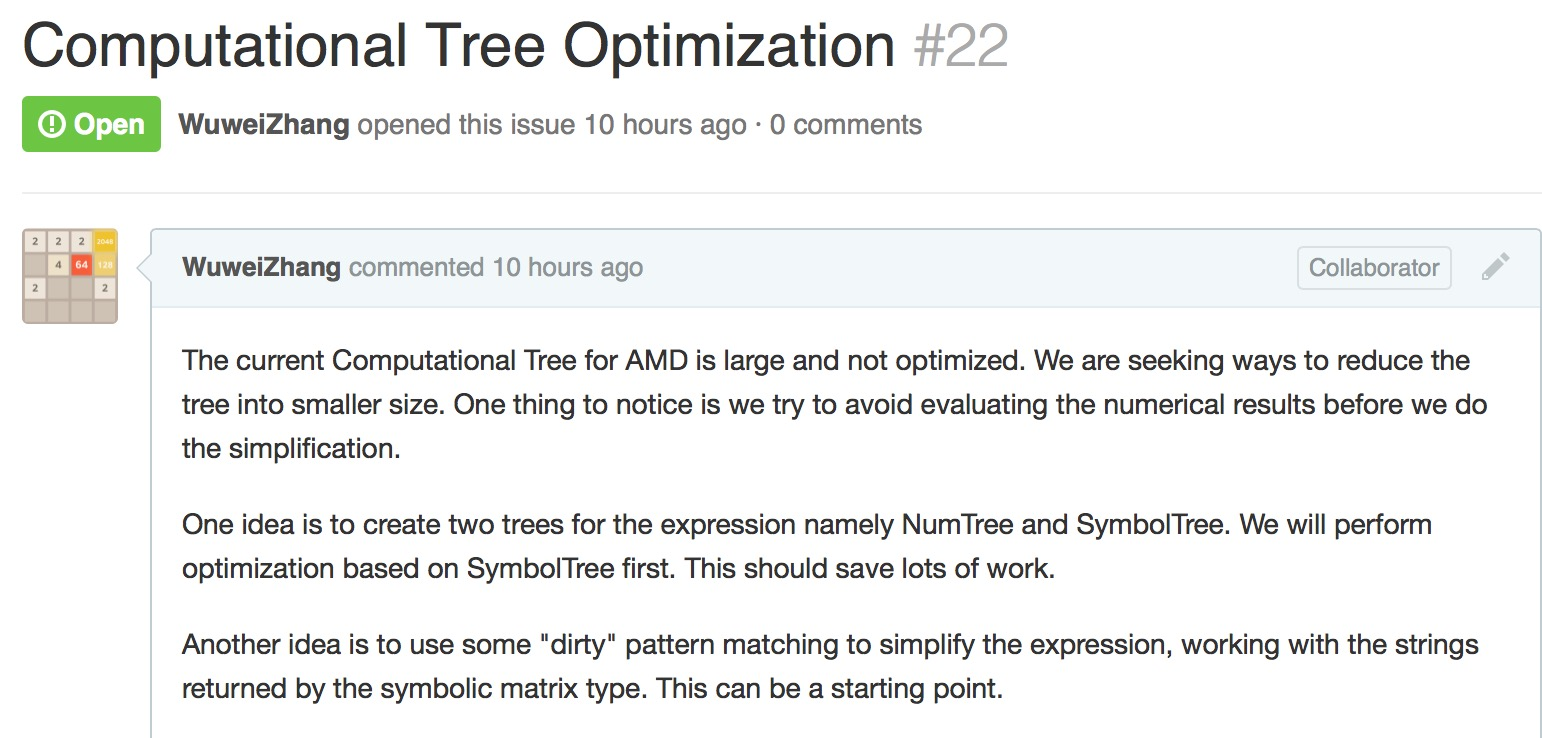
\includegraphics[width=0.7\textwidth]{figs/optimizationIssue.jpg}
\end{center}%
\end{frame}

\begin{frame}[fragile]
\frametitle{Future Works}
%
Anna and Gabriel will work on Python Binding
\begin{center}
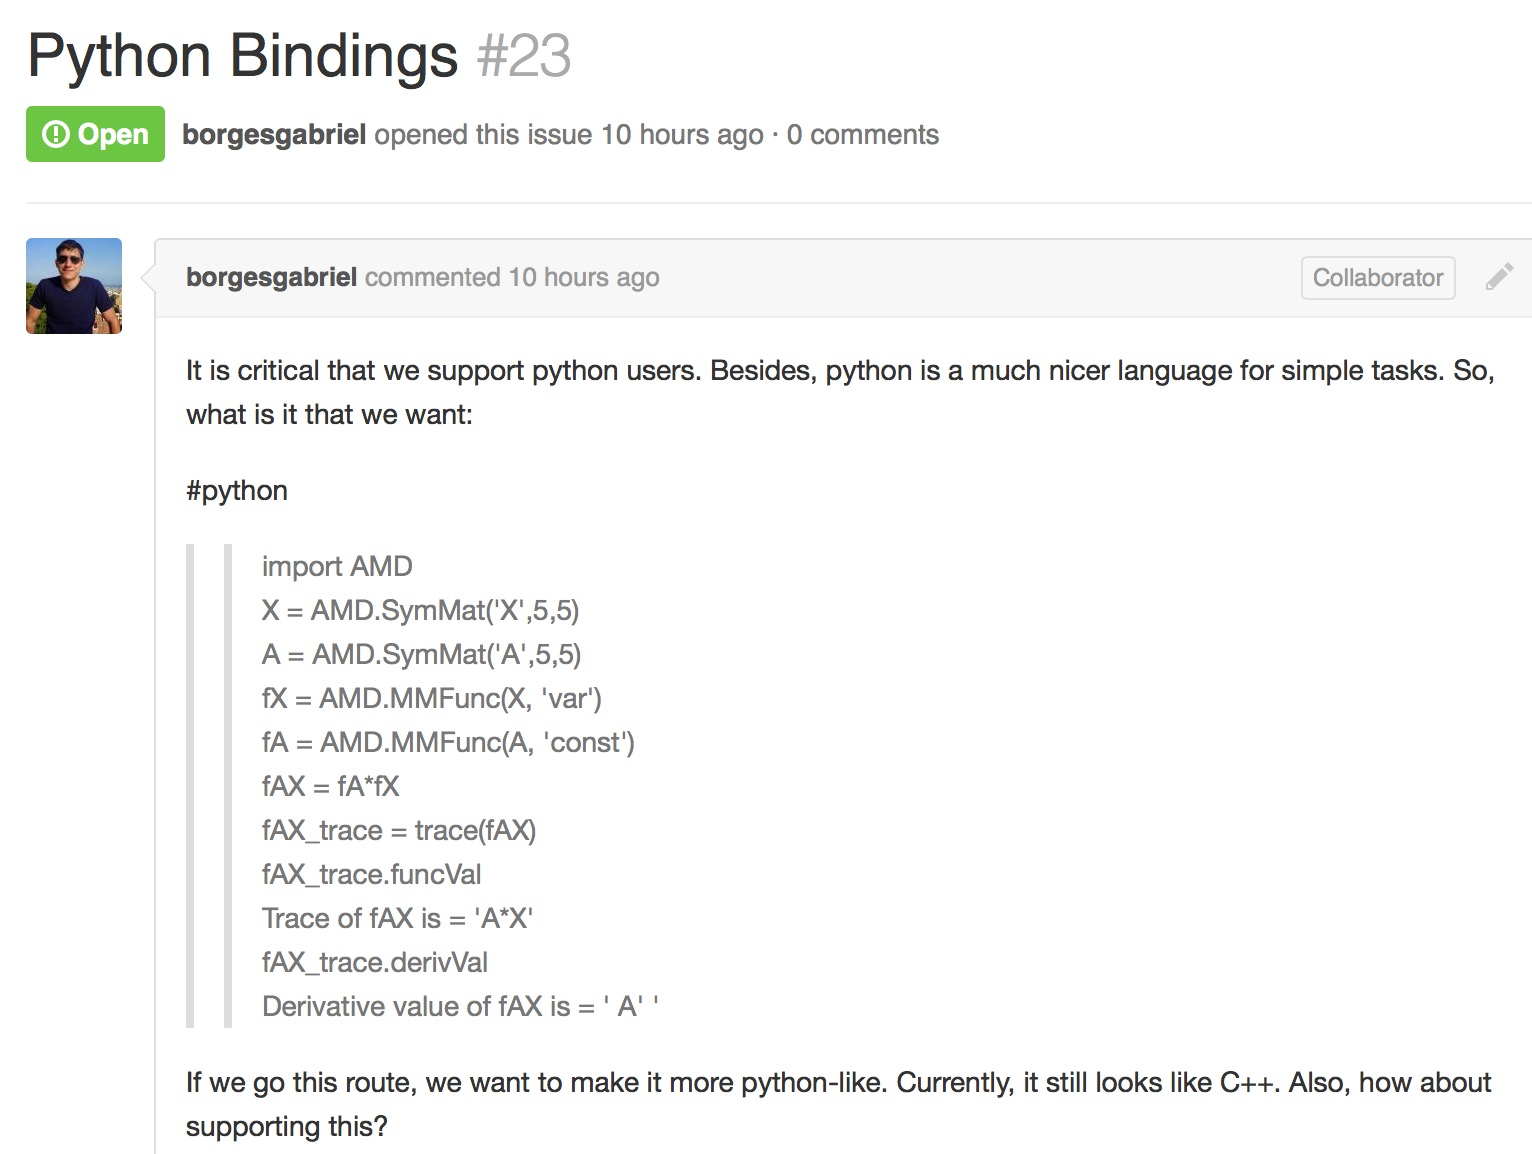
\includegraphics[width=0.7\textwidth]{figs/pythonBindIssue.jpg}
\end{center}%
\end{frame}
